% §1 Introduction --- for the scope §§1-7, which the author fixed as v0.1 on 2026-09-12. Revised the
% same day on the author's comments on the first version: the names "jitter variance" and
% "displacement profile" are this article's, and the profile is explained before it is used; the
% Gaussian is one classical answer among several, not the classical answer; the axiom that
% differs from the causal article is named; Pauwels et al. are described neutrally; "the two
% members" says what they are for; the Wiener algebra is described, not named; "inverts the
% headline" is spelled out; the paragraph on what the line costs is shortened and its details
% left to the remarks of §§4-7; and two related-work paragraphs are added, the scale-space
% axiomatics and the probability theory the class comes from, with references held in the
% library. §1.1 owns the trust base of this scope. Nothing here is shared with the blueprint.
%
% Paper I is cited here (the introduction is one of the three places the reference policy
% allows). Papers VI and VII are not cited.
%
% Two literature claims here are not in the blueprint and were verified by the librarian from the
% held copies on 2026-09-12 (hub note wiki/scale-space-axioms.md carries the anchors):
%   - Iijima's five conditions -- linearity, translation invariance, scale invariance, the
%     (generalized) semigroup property, preservation of positivity -- as reported by Weickert,
%     Ishikawa and Imiya: the held copy is the DIKU technical report (@weickert1997japan), pp. 4-5;
%     the JMIV version cited in the text is not held, so no JMIV page is given.
%   - The Bessel scale-space of Burgeth, Didas and Weickert: multiplier (1 + 4 pi^2 tau^2 |k|^2)^(-t/2)
%     with t the order, p. 86 (tau = 1) and p. 89 (the scaled family); the semigroup runs in t at
%     fixed tau, pp. 88-89; "not scale invariant", p. 89.

\section{Introduction}\label{sec:introduction}

This paper characterizes the spatial scale spaces on the line, the families of smoothing
operators through which an uncommitted observer can measure a signal at every scale, under
translation and reflection symmetry. A front end measures its input before anything is
known about what the signal will contain. It must therefore hold records at every scale,
and it must derive the form of those records from requirements on the measurement process
rather than from a signal model. The classification says which apertures the axioms
admit; whether an aperture creates structure across scale, the non-creation property of
the Gaussian axiomatics, is a further requirement and is outside this paper. In the
Gaussian axiomatics of scale-space theory
\sscite{iijima1962basic,witkin1983scale,koenderink1984structure,babaud1986uniqueness,yuille1986scaling,lindeberg1994scale,florack1997image}
the requirements single out one family of records, the Gaussian smoothings, which solve the
heat equation in scale. Each axiomatics that relaxes one of those requirements arrives at
another class: the scale-invariant recursive filters of \sscite{pauwels1995extended}, the
$\alpha$-scale spaces of \sscite{duits2004axioms}, among them the Poisson scale space of
\sscite{felsberg2001scale}, and the Bessel scale space of \sscite{burgeth2005bessel}. Here
too the answer is a class, arrived at by weakening one requirement, and the Gaussian is one
ray of it.

\emph{The assumption.} The axioms are those of the extended class of Pauwels, Van Gool,
Fiddelaers and Moons \sscite{pauwels1995extended}, with one change. Their recursivity, the
semigroup form of the cascade property $K_sK_t = K_{s+t}$, formalizes ``a measurement of a
measurement is a measurement'' together with a second, tacit assumption: that the composite
depends only on the total amount of scale crossed, so that an increment is determined by
the scale difference alone. This second assumption is the \emph{stationarity of the
increments} in the scale parameter. It is not commutativity, which every family of
convolutions has, and it is what this paper drops. The first assumption is kept, and the
cascade is stated in its weakest defensible form, as a two-parameter \emph{hemigroup},
\[
  \Phi_{s,t}\,\Phi_{r,s} \;=\; \Phi_{r,t}, \qquad 0 \le r \le s \le t
\]
(Figure~\ref{fig:cascade}). The name is that of the probability literature on groups, where
a two-parameter family of measures composing in this way is a convolution hemigroup
(\sscite{heyer1977probability}, Def.~4.6.1, p.~308; \sscite{siebert1982continuous},
p.~365; \sscite{hazod2001stable}, Def.~2.14.16, p.~380); Sato states the same
requirements for a system of probability measures $\{\mu_{s,t}\}$ and constructs from it
an additive process whose increment from $s$ to $t$ has law $\mu_{s,t}$
(\sscite{sato1999levy}, Thm.~9.7, p.~51). Every other axiom --- linearity, translation covariance, reflection symmetry, positivity,
unit mass, continuity, and scale covariance with the relabelling of the scale axis left free
--- is retained, restated as the two-parameter setting requires, with two smaller changes
recorded in Remark~\ref{rem:provenance-pauwels}: the kernels are measures rather than
continuous functions, and positivity is stated as an axiom (\S\ref{sec:axioms}).
This is the same weakening that the companion article on temporal scale space
\sscite{fagerstrom2026hemigroup}, called the causal article in what follows, makes on the
temporal axis,
starting from the semigroup theory of \sscite{fagerstrom2005temporal}.
The two axiom systems differ in exactly one axiom, causality there and reflection symmetry
here, and that one axiom is what excludes the Gaussian aperture in time and admits it in
space.

% Figure: the two readings of the cascade property (semigroup vs hemigroup). Referenced from
% §3.4. Pure TikZ, no external file. Paper I's fig-cascade with this article's letters
% (scales r <= s <= t, the ratio lambda): the pedagogic point is the same, one per panel ---
% (a) semigroup increments are indexed by an AMOUNT of scale, (b) hemigroup increments by
% INTERVALS of the scale axis; composition is the shared content.

\begin{figure}[!htb]
\centering
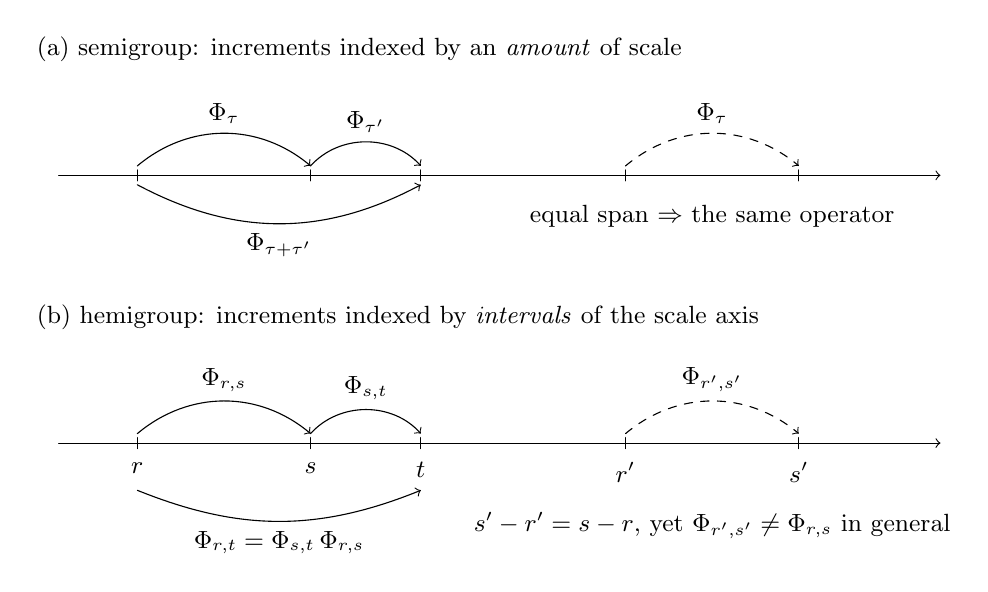
\begin{tikzpicture}[every node/.style={font=\small}, line cap=round]

% ---------- panel (a): semigroup ----------
\begin{scope}[yshift=0cm]
  \node[anchor=west] at (-0.4,1.6) {(a) semigroup: increments indexed by an \emph{amount} of scale};
  \draw[->] (0,0) -- (11.2,0);
  \foreach \x in {1,3.2,4.6,7.2,9.4} \draw (\x,0.07) -- (\x,-0.07);
  \draw[->] (1,0.12) to[bend left=40] node[above] {$\Phi_{\tau}$} (3.2,0.12);
  \draw[->] (3.2,0.12) to[bend left=48] node[above] {$\Phi_{\tau'}$} (4.6,0.12);
  \draw[->] (1,-0.12) to[bend right=28] node[below] {$\Phi_{\tau+\tau'}$} (4.6,-0.12);
  \draw[->,dashed] (7.2,0.12) to[bend left=40] node[above] {$\Phi_{\tau}$} (9.4,0.12);
  \node[anchor=north] at (8.3,-0.25) {equal span $\Rightarrow$ the same operator};
\end{scope}

% ---------- panel (b): hemigroup ----------
\begin{scope}[yshift=-3.4cm]
  \node[anchor=west] at (-0.4,1.6) {(b) hemigroup: increments indexed by \emph{intervals} of the scale axis};
  \draw[->] (0,0) -- (11.2,0);
  \foreach \x/\l in {1/$r$,3.2/$s$,4.6/$t$,7.2/$r'$,9.4/$s'$}
    { \draw (\x,0.07) -- (\x,-0.07); \node[anchor=north] at (\x,-0.12) {\l}; }
  \draw[->] (1,0.12) to[bend left=40] node[above] {$\Phi_{r,s}$} (3.2,0.12);
  \draw[->] (3.2,0.12) to[bend left=48] node[above] {$\Phi_{s,t}$} (4.6,0.12);
  \draw[->] (1,-0.6) to[bend right=22] node[below] {$\Phi_{r,t} = \Phi_{s,t}\,\Phi_{r,s}$} (4.6,-0.6);
  \draw[->,dashed] (7.2,0.12) to[bend left=40] node[above] {$\Phi_{r',s'}$} (9.4,0.12);
  \node[anchor=north] at (8.3,-0.75) {$s'-r' = s-r$, yet $\Phi_{r',s'} \ne \Phi_{r,s}$ in general};
\end{scope}

\end{tikzpicture}
\caption{The two readings of the cascade property. (a)~In the semigroup form the
increment is indexed by an amount of scale: composition adds amounts, and increments of
equal amount are the same operator wherever they act: the axis positions carry no
labels because the operators cannot see them. (b)~In the hemigroup form the increment is
indexed by an interval of the scale axis: composition joins adjacent intervals, and
increments of equal span at different positions need not coincide. The axioms retain what
the two forms share (a measurement of a measurement is a measurement) and drop the
rest.}
\label{fig:cascade}
\end{figure}


\emph{What the class is.} Pauwels et al.\ showed that recursivity and scale invariance alone
do not single out the Gaussian: they admit the extended class $e^{-a|\omega|^\alpha t}$ for
every $\alpha > 0$, with sign-changing kernels beyond $\alpha = 2$, and positivity enters
their derivation only at its end, through the second-moment condition that bounds
$\alpha \le 2$. Under the hemigroup the admissible families are completely characterized
(Theorem~\ref{thm:main-characterization}): in the canonical scale parametrization fixed in
\S\ref{sec:covariance}, they are exactly the families whose kernel at scale $t$ has
transform $e^{-F(t\omega)}$ with
\[
  F(\omega) \;=\; a\,\omega^2 + \int_0^\infty \bigl(1 - \cos\omega x\bigr)\,\frac{k(x)}{x}\,dx,
  \qquad a \ge 0, \quad k \ge 0 \ \text{nonincreasing},
\]
and the pair (gauge, exponent) is unique up to the normalization of the gauge, the gauge
being the scale parametrization that covariance singles out (\S\ref{sec:covariance}).

What the axioms leave free is therefore a number
$a \ge 0$ and a nonincreasing function $k$, and both have a meaning at the kernel. The
kernel at scale $t$ is the law of a random displacement, and the representation says that
the displacement has two independent parts: a Gaussian part of variance $2at^2$, and a sum
of jumps whose intensity at scale $t$ is a dilate of one function. Displacements of size
about $x$ occur at rate $k(x/t)/x$. So at unit scale $k(x)$ is the rate of jumps of
size $x$ weighted by their size, and the whole catalogue stretches with the scale rather
than accumulating linearly in it. We call $k$ the
\emph{displacement profile}. The condition on it, that
larger displacements are never generated at a higher weighted rate than smaller ones, is
what makes the family consistent across scales (Remark~\ref{rem:displacement-dictionary}
develops the reading). In the vocabulary of probability the kernels are the \emph{symmetric
self-decomposable} laws --- the displacements $X$ that shrink into themselves,
$X \stackrel{d}{=} cX + R_c$ with $R_c$ independent, for every $c \in (0,1)$ --- and the
family of their dilates is the marginal family of a self-similar additive process. The
Gaussian scale space is the pair $(a,0)$, the unique member with no jumps, and it is an
extreme ray of the cone the admissible exponents form (Remark~\ref{rem:gaussian-extreme})
rather than the whole answer.

When stationarity of the increments is reimposed, the recovered
subclass is the symmetric stable family, $F(\omega) = |\omega|^\alpha$ with
$0 < \alpha \le 2$ (Corollary~\ref{cor:semigroup-case}), which is the positive part of the
extended class. The members below $\alpha = 2$ are heavy-tailed: their kernels decay like
$|x|^{-1-\alpha}$ and have infinite variance. Those tails are therefore the price of that
tacit assumption rather than of covariance. The class also contains members with all
moments finite. The simplest is the variance-gamma family, with transform
$(1 + t^2\omega^2)^{-\gamma}$. For $\gamma > \tfrac12$ its kernels are the Mat\'ern
covariance functions of spatial statistics
\sscite{whittle1954stationary,guttorp2006studies,porcu2024matern}, of smoothness
$\gamma - \tfrac12$ (the smoothness parameter is positive in the standard form,
\sscite{porcu2024matern}, eq.~(9)); for $\gamma \le \tfrac12$ they are unbounded at the
origin and are densities but not covariance functions. Burgeth, Didas and Weickert
\sscite{burgeth2005bessel} compose the same transforms into their Bessel scale space by
varying the smoothness at fixed range, also in their scaled family (\S~2.4 there); here the
cascade parameter is the range, at fixed smoothness. The family is exhibited in
\S\ref{sec:axioms} beside the Gaussian as the second member on which the axioms are
checked, and the two show what the class must contain: one has no jumps, one has jumps of
every size.

\emph{Which assumption narrows.} Positivity does. In the semigroup setting the class is
one-parameter whether or not positivity is imposed, and positivity only trims the parameter
range. In the hemigroup setting it is what makes a classification possible. Without it the
remaining axioms admit an infinite-dimensional affine family through the Gaussian: the
exponents $\omega^2 + \phi$ for every real, even $\phi$ that is the Fourier transform of an
integrable function and vanishes at the origin. No description of that class by a Gaussian
coefficient and a profile, in the form of Theorem~\ref{thm:main-characterization}, exists
(Proposition~\ref{prop:no-positivity-no-classification}; its construction is the one step
of this paper not machine-checked, \S\ref{sec:machine-checked}). With positivity, the class
collapses to the cone above.

\emph{The route.} The derivation runs in the order of the causal article: the operators
are convolutions, the exponents add along the cascade, covariance forces a similarity form,
and the classification is read off it. Fourier transforms stand in place of Laplace
transforms, and the two theories part company at the transform. The Laplace transform of a
probability measure on the half-line is positive and monotone; the Fourier transform of a
symmetric one can vanish, and the zero set of its exponent can be a lattice
(Lemma~\ref{lem:lattice-zero}). So the exponent exists here only by a nonvanishing lemma
that uses the cascade and continuity together (Lemma~\ref{lem:nonvanishing}). The
relabelling of the scale axis is determined not by the exponent itself but by a smoothed
transmittance, the transform of the kernel averaged against a Gaussian window
(Corollary~\ref{cor:smoothed-transmittance}). And the analysis direction of the
characterization is proved directly from a dilation identity
(Lemma~\ref{lem:selfdecomposable-exponents}), so that the classical description of the
self-decomposable \Levy{} measures is cited for orientation and never used. Each section
records in one remark how its argument relates to the causal one. The kernels from the
origin are absolutely continuous and unimodal about the origin
(Proposition~\ref{prop:kernel-regularity}); the increments between two positive scales need
not be, and can carry an atom. No truncation of the Gaussian is admissible, its transform
changing sign where Lemma~\ref{lem:nonvanishing} requires positivity.

\emph{Relation to the scale-space axiomatics.} The uniqueness of the Gaussian aperture is
the oldest result of the subject, obtained from several axiom systems. Iijima derived it
from linearity, translation and scale invariance, the semigroup and preservation of
positivity \sscite{iijima1962basic,weickert1999linear}, together with a regularity
assumption the derivation leaves implicit, that the transfer function is continuously
differentiable at the origin; without it the Poisson kernel $e^{-t|\omega|}$ satisfies
every listed condition, as Felsberg and Sommer point out
(\sscite{felsberg2004monogenic}, \S~2.1, Thm.~1 and p.~8). The one-dimensional theory of
\sscite{witkin1983scale,babaud1986uniqueness,yuille1986scaling} and Koenderink's causality
\sscite{koenderink1984structure} derive it from non-creation of structure across scale.
Lindeberg derives it from non-enhancement of local extrema
\sscite{lindeberg1990scalespace,lindeberg1994scale,lindeberg2011generalized}, and Florack
from the scale-space differential structure \sscite{florack1992scale,florack1997image}. Each
of these systems imposes, beyond the axioms of \S\ref{sec:axioms}, either the semigroup or
a requirement on how structure may change across scale. What this paper characterizes is
the class from which such a requirement then selects. Within it the Gaussian is the boundary
$\alpha = 2$ of the semigroup slice and the jump-free ray of the cone. The extended class of
\sscite{pauwels1995extended} and the $\alpha$-scale spaces of \sscite{duits2004axioms} keep
the semigroup and weaken other requirements, and they meet the present class in the
symmetric stable family, its semigroup slice. The Bessel scale space of
\sscite{burgeth2005bessel} has the transform of a member, the variance-gamma family, once
it is composed along the range instead of along the smoothness index. The axiomatics of \sscite{alvarez1993axioms}, which
classify the nonlinear evolutions, are orthogonal to the question asked here.

\emph{Relation to probability theory.} The class this paper arrives at is classical in
probability theory. The self-decomposable laws are the class $L$ of \Levy{} and Khintchine, the limit
laws of normalized sums of independent variables, with a developed theory
(\sscite{sato1999levy}, Ch.~3; \sscite{steutel2004infinite}), and the marginal families of
self-similar processes with independent increments are their dilates
(\sscite{sato1999levy}, \S16; the correspondence with its converse construction is
\sscite{sato1991selfsimilar}, Thms.~3.1--3.2, pp.~293--294, in $\RR^d$, and the notion of
self-similarity is Lamperti's \sscite{lamperti1962semistable}).
The tools are classical: Bochner's theorem, that a continuous positive definite function is
the transform of a finite measure, and Schoenberg's, that the exponents are exactly the
functions $\psi$ for which $e^{-\tau\psi}$ is such a transform for every $\tau > 0$
\sscite{berg1975potential,jacob2001pseudo}; the symmetric \Levy--Khintchine representation
of those exponents \sscite{sato1999levy}; \Levy's continuity theorem
\sscite{feller2009introduction}; and Yamazato's unimodality theorem
\sscite{yamazato1978unimodality}. Each is stated with its source where it is used. The
Mat\'ern member is the variance-gamma law of \sscite{madan1990variance}, reviewed in
\sscite{fischer2025variance}. What is new is the derivation of the class from measurement
axioms, the reading of its two parameters as properties of an aperture, and the place the
Gaussian takes in it. The probabilistic facts are cited, not reproven, and
\S\ref{sec:machine-checked} says which of them the verified results use.

The contributions, each with the section that carries it:
\begin{itemize}
\item the characterization of the spatial scale spaces on the line under the hemigroup
  axioms: exactly the symmetric self-decomposable exponents, with the exponent unique and
  the gauge unique up to normalization
  (Theorem~\ref{thm:main-characterization}, \S\ref{sec:characterization});
\item the recovery of the semigroup case from inside the hemigroup theory, the symmetric
  stable family with the bound $\alpha \le 2$ proved from the representation
  (Corollary~\ref{cor:semigroup-case});
\item the proposition that positivity is the narrowing axiom: without it the hemigroup
  axioms admit an infinite-dimensional affine family through the Gaussian
  (Proposition~\ref{prop:no-positivity-no-classification}, \S\ref{sec:axioms}; its
  construction clause rests on the printed proof, \S\ref{sec:machine-checked});
\item the Fourier-side route --- nonvanishing, the lattice zero sets, the smoothed
  transmittance, the dilation argument --- at the places where the line parts from the
  half-line (\S\S\ref{sec:representation}--\ref{sec:covariance});
\item machine-checked proofs of the characterization and of everything it stands on,
  resting on two cited analytic facts (\S\ref{sec:machine-checked}).
\end{itemize}

The paper is about the line, and about the classification. The geometry of the cone and
its extreme rays, the named families inside it (Gaussian, Mat\'ern, symmetric stable),
the scale evolution in generator form, locality, non-creation of local extrema, and the
exact implementation of the cascade by recursive filters are outside it, as are dimension
$d$ and the families covariant only under a discrete group of dilations.
\S\ref{sec:conclusions} names what is left open. Its contribution is mathematical
foundations: no empirical claims about natural signals are made.

The sections follow the derivation in the order above. \S\ref{sec:preliminaries} fixes
the notation, with the table shared with the causal article, and states the Fourier
toolbox with its sources.

\subsection{What is machine-checked}\label{sec:machine-checked}

The characterization and everything it stands on have been formalized in the Lean~4 proof
assistant, on top of its mathematical library Mathlib, and this subsection says which
results, and what they rest on. It is self-contained: nothing below depends on
reading the formal development.

\paragraph{What is proved.} Theorem~\ref{thm:main-characterization} is machine-checked in
all three of its clauses: the construction of a family from an admissible exponent, the
analysis that every family has one, and the uniqueness of the pair (gauge, exponent). The
three are assembled in one declaration, so that the theorem is verified as it is printed.
Everything \S\S\ref{sec:representation}--\ref{sec:covariance} contribute to it is
verified with it. That is the convolution representation and the nonvanishing lemma, the
additivity and infinite divisibility of the exponents with the truncation inequality that
carries the null-array limit (the limit of a sum of many small independent displacements,
Theorem~\ref{thm:increments-levy}), the exclusion of lattice kernels, the
rigidity of the action and the gauge. Of \S\ref{sec:characterization}, the
self-decomposability lemma in all its directions, the semigroup case with its bound
$\alpha \le 2$, the convex cone, and the strict positivity and monotonicity of the
admissible exponents are verified. So are the two toolbox facts that are proved rather than
cited, uniqueness of the Fourier--Stieltjes transform and \Levy's continuity theorem, from
Mathlib's characteristic-function development. Of \S\ref{sec:axioms}, both members are
verified in every axiom, including the continuity axiom at the operator, and the
no-positivity proposition is verified in its positivity equivalence and in its example.

\paragraph{What it rests on.} Two analytic facts are taken from the literature rather than
reproved, and they are the only things the verified characterization assumes beyond the
logical foundations of the proof assistant itself; each is cited with a page reference
checked against the source.
\begin{enumerate}
\item \emph{Bochner's theorem, in the forward direction.} A real-valued continuous positive
definite function with value $1$ at the origin is the cosine transform of a symmetric
probability measure on $\RR$ (\sscite{sato1999levy}, Prop.~2.5, pp.~8--9). This is what turns an
admissible exponent into actual kernels, and it is the only thing the constructive
direction of Theorem~\ref{thm:main-characterization} needs that is not proved here; the
reverse direction is proved.
\item \emph{The symmetric \Levy--Khintchine representation, at its converse and its
uniqueness clauses.} Every pair $(a,\nu)$ with $a \ge 0$ and
$\int (1 \wedge x^2)\,\nu(dx) < \infty$ defines a member of $\NDs$, the class of symmetric continuous negative definite functions,
and the pair of a member
is unique (\sscite{sato1999levy}, Thm.~8.1, pp.~37--38). The converse is used by the
construction, the uniqueness by the analysis direction of
Lemma~\ref{lem:selfdecomposable-exponents} and by nothing else the theorem needs.
\end{enumerate}
Table~\ref{tab:trust-base} lists every cited fact of the paper with the results that use it
directly; the dependency graph of the repository carries the transitive picture.

\begin{table}[!htb]
\centering
\caption{The cited facts and their direct uses. A result not listed uses no cited fact
directly; it may use one through a listed result, and the dependency graph of the
repository shows which. Cited for orientation and used by no proof: Schoenberg's theorem
(Proposition~\ref{prop:fourier-toolbox}(2)), the existence half of its clause (3) and its
closure clause (4), the classical description of the self-decomposable \Levy{} measures
(Proposition~\ref{prop:sd-exponents}), and the closed form of the variance-gamma density.}
\label{tab:trust-base}
\small
\setlength{\tabcolsep}{5pt}
\begin{tabular}{@{}lll@{}}
\toprule
cited fact & clause used & used directly by \\
\midrule
Bochner's theorem & forward direction & Thm.~\ref{thm:increments-levy}, last sentence; Thm.~\ref{thm:main-characterization}, construction \\
symmetric \Levy--Khintchine & converse & the same two \\
representation & uniqueness & Thm.~\ref{thm:increments-levy}, the pair; Lemma~\ref{lem:selfdecomposable-exponents}, analysis \\
absolute continuity in class $L$ & as stated, $d = 1$ & Prop.~\ref{prop:kernel-regularity} \\
Yamazato's unimodality theorem & symmetric case & Prop.~\ref{prop:kernel-regularity} \\
\bottomrule
\end{tabular}
\end{table}
The second fact carries one step beyond its
pages: its converse is admitted for \Levy{} measures already folded onto $(0,\infty)$, where
the source states the representation on the punctured line with a centering term, and the
folding reduction of \S\ref{sec:preliminaries}, elementary and written out there, sits
inside the admitted statement rather than beside it. The first fact carries nothing beyond
its pages; its admitted hypotheses are stronger than the source's.

The regularity of the kernels, Proposition~\ref{prop:kernel-regularity}, rests on two
further cited facts, used by that proposition alone and by nothing the characterization
needs: that a nondegenerate self-decomposable law is absolutely continuous
(\sscite{sato1999levy}, Thm.~27.13, p.~181) and that a law of class $L$ is unimodal
(\sscite{yamazato1978unimodality}, Thm.~1, p.~523). The one admitted statement that
carries them adds two steps beyond the pages, the symmetric rider that places the mode at
the origin and the choice of a named density whose monotonicity holds pointwise on the open
half-line. The hypothesis check, that the kernels from the origin are nondegenerate and
self-decomposable, is proved. Nothing is claimed about the density's value at the
origin, where it may be unbounded. The two members of \S\ref{sec:axioms} use no cited fact:
the moments of the Mat\'ern member are verified by the Gaussian-mixture argument printed in
the appendix, on Lean core.

\paragraph{Why these and not more.} The classical route to the characterization passes
through the closure of $\NDs$ under pointwise limits and the existence half of the
\Levy--Khintchine representation, and neither is used: the null-array limit extracts the
representation of an increment directly, before any limit is taken, and the profile form is
proved from the dilation identity where the half-line development cites it. So the trust
base is narrower than the naive route by two clauses of the toolbox, and narrower than the
causal article's at the one place where that article carries the classical
self-decomposability theorem. The same policy runs in the other direction: classical
results of structural rather than analytic character are proved, not cited: the
convolution representation of \S\ref{sec:representation}, classically Wendel's theorem, is
proved from scratch, and the quadratic growth bound that gives $\alpha \le 2$ is three lines
from the truncation split rather than a cited estimate.

\paragraph{What is not formalized.} One thing in the scope of this paper, and the text
names it where it occurs. The first clause of
Proposition~\ref{prop:no-positivity-no-classification}, the construction of the signed
family and the verification of the axioms for it, rests on the printed proof: the library
used carries the $\Lone$ Fourier transform but not the algebra of such transforms as a
Banach algebra, and a route through the convolution operators has been estimated and not
carried out. Every other numbered statement is machine-checked, including both members of
\S\ref{sec:axioms} at every axiom, the variance and the moments. The closed form of the
Mat\'ern member's kernel is cited there and is not a statement of this paper.

\paragraph{Where to look.} The development and its axiom ledger, with page-verified
citations for every cited interface, are at the repository accompanying this paper,
\url{https://github.com/danielfagerstrom/spatial-hemigroup-scale-space-kernels}: the Lean
modules that the statements of this paper rest on, the trust boundary and the ledger, and
the sources of the blueprint chapters behind
\S\ref{sec:preliminaries}--\S\ref{sec:characterization}, in which the declaration behind
each numbered statement is named in a \texttt{\char`\\lean} tag on that statement. It is an
export, at the revision named in its changelog, from the development repository, which also
holds the material of two further articles. The toolchain is pinned in-tree --- Lean~4
\texttt{v4.31.0}, Mathlib \texttt{v4.31.0}, and the shared library \texttt{ScaleSpaceCore}
at its tag \texttt{v0.2.0} --- so the verification is reproducible with one command,
\texttt{lake build} in \texttt{Formalization/}. A second,
\texttt{lake env lean CIAxiomGuard.lean}, prints the axiom usage of every named declaration,
to be read against the trust-boundary file beside it. On the declaration
\texttt{SpatialLine.main\_characterization} it prints Lean's three logical axioms and the
three names of the two cited facts above, and nothing else:
\begin{verbatim}
'SpatialLine.main_characterization' depends on axioms: [propext,
 Classical.choice, Quot.sound,
 SpatialLine.fourier_toolbox_bochner_symm,
 SpatialLine.fourier_toolbox_levy_converse,
 SpatialLine.fourier_toolbox_levy_unique]
\end{verbatim}
